\ylDisplay{Vastlaliug} % Ülesande nimi
{Moorits Mihkel Muru} % Autor
{lõppvoor} % Voor
{2017} % Aasta
{G 1} % Ülesande nr.
{2} % Raskustase
{
% Teema: Dünaamika
\ifStatement
\begin{wrapfigure}[5]{r}{0.45\linewidth}
	\vspace{-5pt}
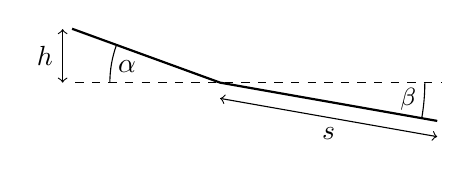
\begin{tikzpicture}[scale=0.4]
% Nõlv
\draw [thick] (0,0) -- (160:5);
\draw [thick] (0,0) -- (-10:7);

% Nurgad
\draw [dashed] (-4.6,0) -- (7,0);
\draw (160:3.5) arc (160:180:3.5) node at (170:3) {\(\alpha\)};
\draw (0:6.5) arc (0:-10:6.5) node at (-5:6) {\small\(\beta\)};

% Suurused
\draw [<->] (-5,0) -- (-5,1.7) node[pos=0.5, left] {\(h\)};
\draw [<->, yshift=-0.5cm] (0,0) -- (-10:7) node[pos=0.5, below] {\(s\)};	
\end{tikzpicture}
%\caption{Künka läbilõige} \label{liug}
\end{wrapfigure}

Juss leidis vastlaliu laskmiseks künka, mille läbilõige koosneb kahest sirglõigust, nagu näha joonisel, edasi on horisontaalne maa. Esimese nõlvaosa kõrgus on \(h=\SI{2}{\meter}\) ja selle kalle \(\alpha=\ang{20}\), teise osa pikkus on \(s=\SI{20}{\meter}\) ja kalle \(\beta=\ang{5}\). Jussi mass koos kelguga on \(m=\SI{47}{\kilogram}\) ja hõõrdetegur lume ja kelgu vahel on \(\mu=\num{0.08}\), raskuskiirendus \(g=\SI{9.8}{\meter\per\second\squared}\). Leidke, kui pikk on Jussi vastlaliug.
\fi


\ifHint
Hõõrdejõu tõttu kulutatud energia sõltub läbitud teepikkusest ja selle kaldest, potentsiaalse energia vahe sõltub kõrguse muudust.
\fi


\ifSolution
Hõõrdejõu tõttu kulutatud energia sõltub läbitud teepikkusest ja selle kaldest, potentsiaalse energia vahe sõltub kõrguse muudust. Esimesel lõigul vabaneb potentsiaalne energia \(E_1 = mgh\) ja hõõrdejõu mõjul liikumiseks kaotatakse energia
\[
A_1 = \mu \cdot mg\cos\alpha \cdot \frac{h}{\sin\alpha} = \mu mgh \cot\alpha.
\]
Teisel lõigul vabaneb potentsiaalne energia \(E_2 = mgs \sin\beta\) ja hõõrdejõu tõttu kaotatakse energia
\[
A_2 = \mu \cdot mg \cos \beta \cdot s = \mu mgs \cos \beta.
\]
Seega nõlva lõppedes on kelgutajal alles kineetiline energia
\begin{align*}
\Delta E &= E_1 - A_1 + E_2 - A_2 = \\
&= mgh(1-\mu\cot\alpha) + mgs(\sin\beta - \mu\cos\beta) = \SI{787.4}{\joule} \, .
\end{align*}
Tasase maa peal enam potentsiaalset energiat ei vabane, aga kineetiline energia väheneb hõõrdumise tõttu. Kelk libiseb tasase maa peal
\begin{align*}
l = \frac{\Delta E}{F_h} = \frac{\Delta E}{\mu mg} = \SI{21.4}{\meter} \, .
\end{align*}
Seega kogu vastlaliu pikkus on
\[
\frac{h}{\sin\alpha} + s + l = \SI{47.2}{\meter}.
\]
\fi


\ifEngStatement
% Problem name: Fastelavn slide
\begin{wrapfigure}[5]{r}{0.45\linewidth}
	\vspace{-5pt}
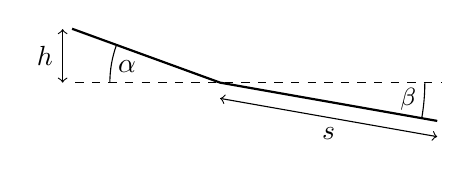
\begin{tikzpicture}[scale=0.4]
% Nõlv
\draw [thick] (0,0) -- (160:5);
\draw [thick] (0,0) -- (-10:7);

% Nurgad
\draw [dashed] (-4.6,0) -- (7,0);
\draw (160:3.5) arc (160:180:3.5) node at (170:3) {\(\alpha\)};
\draw (0:6.5) arc (0:-10:6.5) node at (-5:6) {\small\(\beta\)};

% Suurused
\draw [<->] (-5,0) -- (-5,1.7) node[pos=0.5, left] {\(h\)};
\draw [<->, yshift=-0.5cm] (0,0) -- (-10:7) node[pos=0.5, below] {\(s\)};	
\end{tikzpicture}
%\caption{Künka läbilõige} \label{liug}
\end{wrapfigure}
Juss found a hill for Fastelavn (a carnival tradition and holiday in Northern Europe) sliding. The hill’s cross-cut consists of two line segments, as shown in the figure. After the hill there is a horizontal ground. The height of the hill’s first part is \(h=\SI{2}{\meter}\) and its inclination is \(\alpha=\ang{20}\). The length of the second part is \(s=\SI{20}{\meter}\) and inclination \(\beta=\ang{5}\). The mass of Juss and the sledge is \(m=\SI{47}{\kilogram}\) and coefficient of friction between the snow and the sledge is \(\mu=\num{0.08}\), gravitational acceleration is \(g=\SI{9.8}{\meter\per\second\squared}\). Find how long is Juss’s slide.
\fi


\ifEngHint
The energy spent due to the friction force depends on the distance covered and its inclination, the difference of the potential energy depends on the change of height.
\fi


\ifEngSolution
The energy spent due to frictional force depends on the distance covered and on the road’s inclination, the difference of potential energy depends on the height’s change. On the first segment potential energy \(E_1 = mgh\) is released and on the account of friction energy \( A_1 = \mu \cdot mg\cos\alpha \cdot \frac{h}{\sin\alpha} = \mu mgh \cot\alpha \) is lost during movement. On the second segment potential energy \(E_2 = mgs \sin\beta\) is released and due to friction energy \( A_2 = \mu \cdot mg \cos \beta \cdot s = \mu mgs \cos \beta \) is lost. Thus, at the end of the hill Juss has the kinetic energy
\begin{align*}
\Delta E &= E_1 - A_1 + E_2 - A_2 = \\
&= mgh(1-\mu\cot\alpha) + mgs(\sin\beta - \mu\cos\beta) =  \SI{787.4}{\joule} \, .
\end{align*} 
left. On a flat ground no more potential energy is released but kinetic energy decreases due to friction. The distance the sledge slides on the flat ground
\begin{align*}
l = \frac{\Delta E}{F_h} = \frac{\Delta E}{\mu mg} = \SI{21.4}{\meter} \, .
\end{align*} 
Thus the whole length of the Fastelavn slide is \(\frac{h}{\sin\alpha} + s + l = \SI{47.2}{\meter}\).
\fi
}